%%%%%%%%%%%%%%%%%%%%%%%%%%%%%%%%%%%%%%%%%
% Wenneker Article
% LaTeX Template
% Version 2.0 (28/2/17)
%
% This template was downloaded from:
% http://www.LaTeXTemplates.com
%
% Authors:
% Vel (vel@LaTeXTemplates.com)
% Frits Wenneker
%
% License:
% CC BY-NC-SA 3.0 (http://creativecommons.org/licenses/by-nc-sa/3.0/)
%
% Adapted for COMS30007 by Carl Henrik Ek
%
%%%%%%%%%%%%%%%%%%%%%%%%%%%%%%%%%%%%%%%%%

%----------------------------------------------------------------------------------------
%	PACKAGES AND OTHER DOCUMENT CONFIGURATIONS
%----------------------------------------------------------------------------------------

\documentclass[10pt, a4paper, twocolumn]{article} % 10pt font size (11 and 12 also possible), A4 paper (letterpaper for US letter) and two column layout (remove for one column)

%%%%%%%%%%%%%%%%%%%%%%%%%%%%%%%%%%%%%%%%%
% Wenneker Article
% Structure Specification File
% Version 1.0 (28/2/17)
%
% This file originates from:
% http://www.LaTeXTemplates.com
%
% Authors:
% Frits Wenneker
% Vel (vel@LaTeXTemplates.com)
%
% License:
% CC BY-NC-SA 3.0 (http://creativecommons.org/licenses/by-nc-sa/3.0/)
%
% Adapted for COMS30007 by Carl Henrik Ek
%
%%%%%%%%%%%%%%%%%%%%%%%%%%%%%%%%%%%%%%%%%

%----------------------------------------------------------------------------------------
%	PACKAGES AND OTHER DOCUMENT CONFIGURATIONS
%----------------------------------------------------------------------------------------

\usepackage[english]{babel} % English language hyphenation

\usepackage{microtype} % Better typography

\usepackage{amsthm} % Math packages for equations
\usepackage{amsmath}
\usepackage{amssymb}
\usepackage{mathtools}
\usepackage{bm}
\usepackage{xfrac}
\usepackage{resizegather}
\usepackage[backend=bibtex,style=numeric]{biblatex}



\usepackage[svgnames]{xcolor} % Enabling colors by their 'svgnames'

\usepackage[hang, small, labelfont=bf, up, textfont=it]{caption} % Custom captions under/above tables and figures

\usepackage{booktabs} % Horizontal rules in tables

\usepackage{lastpage} % Used to determine the number of pages in the document (for "Page X of Total")

\usepackage{graphicx} % Required for adding images

\usepackage{enumitem} % Required for customising lists
\setlist{noitemsep} % Remove spacing between bullet/numbered list elements

\usepackage{sectsty} % Enables custom section titles
\allsectionsfont{\usefont{OT1}{phv}{b}{n}} % Change the font of all section commands (Helvetica)

%----------------------------------------------------------------------------------------
%	MARGINS AND SPACING
%----------------------------------------------------------------------------------------

\usepackage{geometry} % Required for adjusting page dimensions

\geometry{
	top=1cm, % Top margin
	bottom=1.5cm, % Bottom margin
	left=2cm, % Left margin
	right=2cm, % Right margin
	includehead, % Include space for a header
	includefoot, % Include space for a footer
	%showframe, % Uncomment to show how the type block is set on the page
}

\setlength{\columnsep}{7mm} % Column separation width

%----------------------------------------------------------------------------------------
%	FONTS
%----------------------------------------------------------------------------------------

\usepackage[T1]{fontenc} % Output font encoding for international characters
\usepackage[utf8]{inputenc} % Required for inputting international characters

\usepackage{XCharter} % Use the XCharter font

%----------------------------------------------------------------------------------------
%	HEADERS AND FOOTERS
%----------------------------------------------------------------------------------------

\usepackage{fancyhdr} % Needed to define custom headers/footers
\pagestyle{fancy} % Enables the custom headers/footers

\renewcommand{\headrulewidth}{0.0pt} % No header rule
\renewcommand{\footrulewidth}{0.4pt} % Thin footer rule

\renewcommand{\sectionmark}[1]{\markboth{#1}{}} % Removes the section number from the header when \leftmark is used

%\nouppercase\leftmark % Add this to one of the lines below if you want a section title in the header/footer

% Headers
\lhead{} % Left header
\chead{\textit{\thetitle}} % Center header - currently printing the article title
\rhead{} % Right header

% Footers
\lfoot{} % Left footer
\cfoot{} % Center footer
\rfoot{\footnotesize Page \thepage\ of \pageref{LastPage}} % Right footer, "Page 1 of 2"

\fancypagestyle{firstpage}{ % Page style for the first page with the title
	\fancyhf{}
	\renewcommand{\footrulewidth}{0pt} % Suppress footer rule
}

%----------------------------------------------------------------------------------------
%	TITLE SECTION
%----------------------------------------------------------------------------------------

\newcommand{\authorstyle}[1]{{\large\usefont{OT1}{phv}{b}{n}\color{DarkRed}#1}} % Authors style (Helvetica)

\newcommand{\institution}[1]{{\footnotesize\usefont{OT1}{phv}{m}{sl}\color{Black}#1}} % Institutions style (Helvetica)

\usepackage{titling} % Allows custom title configuration

\newcommand{\HorRule}{\color{DarkGoldenrod}\rule{\linewidth}{1pt}} % Defines the gold horizontal rule around the title

\pretitle{
	\vspace{-20pt} % Move the entire title section up
	\fontsize{32}{36}\usefont{OT1}{phv}{b}{n}\selectfont % Helvetica
	\color{DarkRed} % Text colour for the title and author(s)
}

\posttitle{\par\vskip 5pt} % Whitespace under the title

\preauthor{} % Anything that will appear before \author is printed

\postauthor{ % Anything that will appear after \author is printed
	\vspace{2pt} % Space before the rule
	\par\HorRule % Horizontal rule after the title
	\vspace{1pt} % Space after the title section
}

%----------------------------------------------------------------------------------------
%	ABSTRACT
%----------------------------------------------------------------------------------------

\usepackage{lettrine} % Package to accentuate the first letter of the text (lettrine)
\usepackage{fix-cm}	% Fixes the height of the lettrine

\newcommand{\initial}[1]{ % Defines the command and style for the lettrine
	\lettrine[lines=3,findent=4pt,nindent=0pt]{% Lettrine takes up 3 lines, the text to the right of it is indented 4pt and further indenting of lines 2+ is stopped
		\color{DarkGoldenrod}% Lettrine colour
		{#1}% The letter
	}{}%
}

\usepackage{xstring} % Required for string manipulation

\newcommand{\lettrineabstract}[1]{
	\StrLeft{#1}{1}[\firstletter] % Capture the first letter of the abstract for the lettrine
	\initial{\firstletter}\textbf{\StrGobbleLeft{#1}{1}} % Print the abstract with the first letter as a lettrine and the rest in bold
}

%----------------------------------------------------------------------------------------
%	BIBLIOGRAPHY
%----------------------------------------------------------------------------------------

% Use the bibtex backend with the authoryear citation style (which resembles APA)

\addbibresource{example.bib} % The filename of the bibliography

\usepackage[autostyle=true]{csquotes} % Required to generate language-dependent quotes in the bibliography
 % Specifies the document structure and loads requires packages

%\setlength{\parindent}{0pt}

\usepackage{lipsum}
\def \vecY {\textbf{Y}}

%----------------------------------------------------------------------------------------
%	ARTICLE INFORMATION
%----------------------------------------------------------------------------------------

\title{Inference} % The article title

\author{
	\authorstyle{James O'Reilly\textsuperscript{1},  Adam Pluck\textsuperscript{2} and Jake Witter\textsuperscript{3}} % Authors
	\newline\newline % Space before institutions
	\textsuperscript{1}\institution{35055},  % Institution 1
	\textsuperscript{2}\institution{34013},  % Institution 2
	\textsuperscript{3}\institution{35445}
}

\date{} % Add a date here if you would like one to appear underneath the title block, use \today for the current date, leave empty for no date

\def \qx   {$q(\textbf{x})$}
\def \px   {$p(\textbf{x})$}
%----------------------------------------------------------------------------------------

\begin{document}

\maketitle % Print the title

\thispagestyle{firstpage} % Apply the page style for the first page (no headers and footers)

%----------------------------------------------------------------------------------------
%	ABSTRACT
%----------------------------------------------------------------------------------------
\lettrineabstract{In machine learning, it is often the case that the evidence is computationally or analytically intractable. In these cases, different methods can be used to sample from or approximate our posterior. This report outlines and compares 3 different approaches, in the context of recovering a noisy image. In this case, the original image is our posterior that we are attempting to sample from.}\\


%----------------------------------------------------------------------------------------
%	ARTICLE CONTENTS
%----------------------------------------------------------------------------------------

\noindentThroughout Throughout the report, we use Figure \ref{fig:Haunter} - a grayscale 128 x 128 pixel image - as the clean image that we are trying to recover.

\begin{figure}[h]
    \centering
    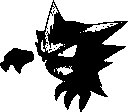
\includegraphics[width = 4cm, scale= 0.2]{images/H.jpg}
    \caption{Haunter}
    \label{fig:Haunter}
\end{figure}

\noindent\textbf{Question 1}\\
When implementing ICM, a few approaches present themselves, some of which are crude and some of which are more sophisticated. Originally, the implementation of ICM that we chose was quite crude. When classifying a pixel based on its neighbours, we merely counted the number of black or white pixels in the neighbourhood and assigned the pixel to the majority class. There are a few issues with this approach: we do not have the ability to place a weighting on the neighbouring pixels. Furthermore, this approach does not account for the centre pixel from the previous iteration and so only takes into account the neighbouring pixels and not the pixel value itself.

In light of these flaws, we implemented a more sophisticated classification method, based on the energy function defined in Bishop \cite{Bishop:2006ui}.

\begin{equation}
    E(\mathbf{x}, \mathbf{y}) = - \beta \sum_{(i,j)}x_i x_j - \eta \sum_{i}x_i y_i
\end{equation}

The $\beta$ and $\eta$ parameters allow for a weight to be placed on either the neighbouring pixels or the centre pixel based on the preferences or beliefs about the image. If we had some prior assumptions about the nature of the image, these could be encoded in the ICM function. For example, if we believed the image had mostly horizontal and vertical lines, we would apply more weight to the pixels above and below the current pixel, and weight less heavily in the direction of the diagonals.

Finally, one must decide how to classify a given pixel when entropy is maximum ($H(x) = 1$). If the pixel is classified as white (without loss of generality) then this would cause a white trend to propagate through the chain of dependent probabilities and therefore through the image over time. This behaviour is evident when comparing the images in figure \ref{fig:chessboard}. ICM will then terminate once the image is fully white (with the exception of a few edge pixels). Therefore, in the case of max entropy it is best to leave the pixel unchanged from the previous iteration (This is under the assumption that when the image was corrupted, each pixel is flipped with probability < 0.5). This approach ensures that the image terminates in a reasonable state.


\begin{figure}
    \centering
    \subfloat{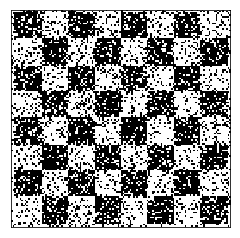
\includegraphics[width = 3.5cm]{images/chessSNP.png}} 
    \qquad
    \subfloat{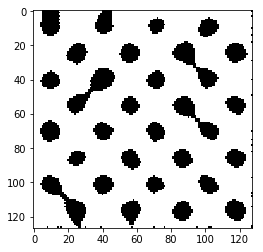
\includegraphics[width = 3.5cm]{images/chessboardfinal.png}} 
    \caption{Results of a poor ICM function on an image of a chessboard after seven iterations. Note how white propagates through the image.}
    \label{fig:chessboard}%
\end{figure}

\begin{figure}
    \centering
    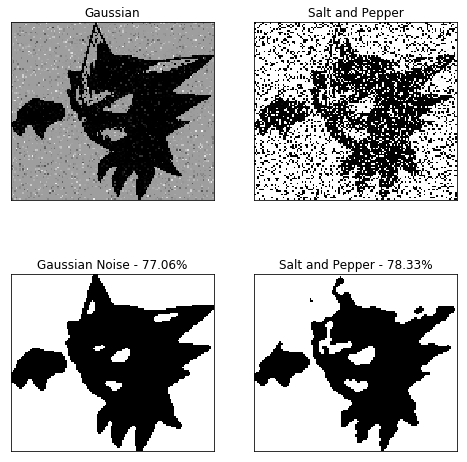
\includegraphics[width = 0.48\textwidth]{images/ICMFinal.png}
    \caption{ICM results for different noises, with percentage match. Prop = 0.2, VarSigma = 0.2}
    \label{fig:ICMfinal}
\end{figure}

Looking at figure \ref{fig:MethodComparisonChanges}, it is clear that ICM makes the vast majority of its changes in the first iteration and then quickly reaches a local maximum. In terms of accuracy, ICM fails to maintain the finer details of the image but preserves the general structure rather well while eliminating the salt and pepper noise. 

ICM can only optimise the posterior $p(\mathbf{y}|\mathbf{x})$ locally and cannot guarantee that a global maximum will be found. The posterior distribution can be viewed as a manifold. If this manifold has many local maxima, then ICM will be sensitive to initialisation and may perform poorly. An intuitive way to think about this problem is to imagine the movement of a ball on a surface with many sinks, and we want the ball to settle in the deepest sink. Once the ball rolls into one of the sinks (a local minimum) then it cannot leave this local minimum and find the global minimum. The ball will reach different minima dependent on where on the surface it is originally placed. The same problem arises when trying to maximise the posterior in ICM. Random restarts may mitigate the problem and for this reason it may be beneficial to perform ICM by visiting pixels randomly and trying out different initialisation configurations.

Unlike Gibbs sampling, ICM is guaranteed to quickly converge to a local maximum. This is a result of the fact that ICM monotonically increases the estimate of the posterior $p(\mathbf{y}|\mathbf{x})$. Given this fact, and using that the value of this posterior is bounded above by $1$, the Monotone Convergence Theorem can be used to prove that ICM will always converge to a local maximum.\\ 

\noindent\textbf{Question 2}\\
In an attempt to obtain better results, we implemented the Gibbs Sampling Ising Model. This is an example of a Markov Chain Monte Carlo method. After implementing the algorithm, one must decide how to implement the prior and likelihood term from the equation. The prior belief is simply that the value of a pixel is similar to its neighbours, and the likelihood gives that $\textbf{y}_i$ and $\textbf{x}_i$ should be similar. 


For the likelihood function, we used Equation \ref{eq:GibbLikelihood}.
\begin{equation}
    p(\textbf{y}_i |\ \textbf{x}_i) = \exp(\eta \mathcal{L}_i (\textbf{x}_i, \textbf{y}_i))
    \label{eq:GibbLikelihood}
\end{equation}
Intuitively, $\mathcal{L}_i$ should be defined so that the function would give a larger value for more similar $\textbf{x}_i$ and $\textbf{y}_i$. One such function that satisfies this requirement is 

\begin{equation}
    \mathcal{L}_i = \frac{1}{|\textbf{x}_i - \textbf{y}_i|}
\end{equation}

As we cannot divide by zero, $\textbf{x}_i$ and $\textbf{y}_i$ should never be equal. To avoid this, we use values of 1.1. and -0.1 for $\textbf{x}_i$ in place of 1 and 0.

The prior used is defined in equation \ref{eq:GibbPrior}.
\begin{equation}
    \label{eq:GibbPrior}
    p(x_i = 1, \textbf{x}_\mathcal{N}_i) = \exp\left({\beta \sum_{j\in\mathcal{N}_i} 1 * \textbf{x}_ j}\right)
\end{equation}

Figure \ref{fig:GibbDifferentLevels} shows the performance on the images with Gaussian and salt and pepper noise, with different noise levels. It performs much better with Gaussian noise than with salt and pepper noise.

One noteworthy point is that we use 'percentage match to the clean image' as our measure, in an attempt to evaluate the effectiveness of the denoising. However, this doesn't actually seem like a great metric. For example, an all white image would give (in our case) a percentage match of upwards of 50\% - we would much rather be evaluating our results with some kind of measure of 'how much a person thinks it look like the original'. Quantifying this is clearly somewhere between very hard and impossible, so percentage match is what we have gone with. For example, in Figure \ref{fig:GibbDifferentLevels}, the bottom right image is bordering on unrecognisable but only scores 7\% less than the top right, which does look considerably better. \\

\begin{figure}
    \centering
    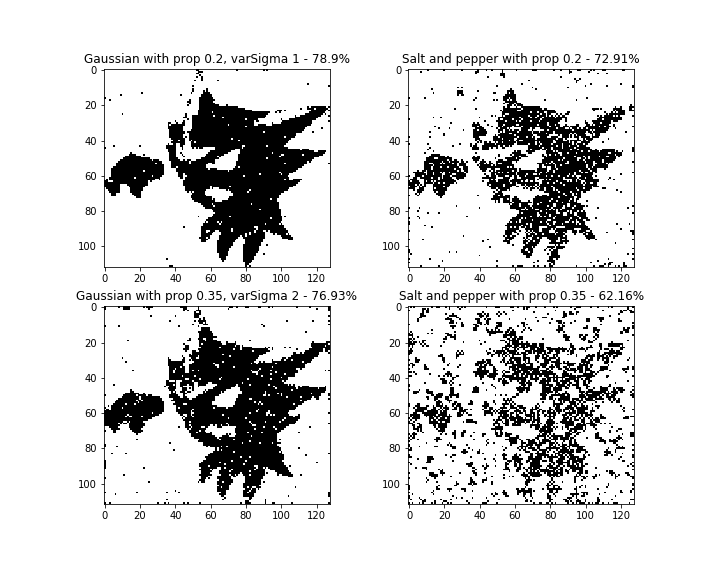
\includegraphics[width=0.48\textwidth]{images/GibbGridDifferentLevels.png}
    \caption{Gibbs results from noise different levels, with percentage match}
    \label{fig:GibbDifferentLevels}
\end{figure}

\noindent\textbf{Question 3} \\
Two different methods were implemented to change the order in which pixels are visited. The first approach is to shuffle the order in which each pixel is visited for each iteration. With this approach each pixel is still visited once per iteration. This approach has a negligible effect on the performance of the Gibbs sampler, as can be seen in Figure \ref{fig:GibbOrderComp}, but in theory removes any systematic bias that results from visiting pixels in a fixed systematic order each time.

The second approach involves fully randomising which pixels are visited. It is therefore extremely unlikely that each pixel is visited each iteration. This does take longer to converge than our other methods, but ultimately converges to the same result, shown in Figure \ref{fig:GibbOrderComp}.

Figure \ref{fig:GibbOrderHaunter} shows the results of these approaches with their percentage match to the original image. After 50 iterations they give a similar result, and the difference in their matches is effectively negligible and a result of the randomness in the process.\\\\
\begin{figure}
    \centering
    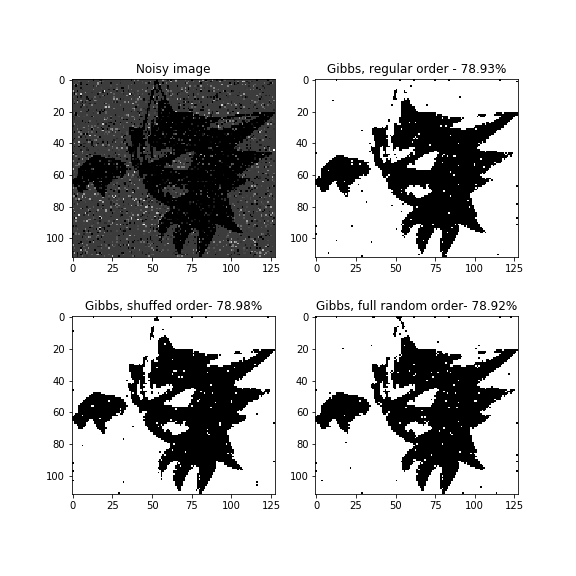
\includegraphics[width=0.48\textwidth]{images/HaunterGibbGridGuassian.png}
    \caption{Results from running Gibbs using different pixel ordering}
    \label{fig:GibbOrderHaunter}
\end{figure}
\begin{figure}
    \centering
    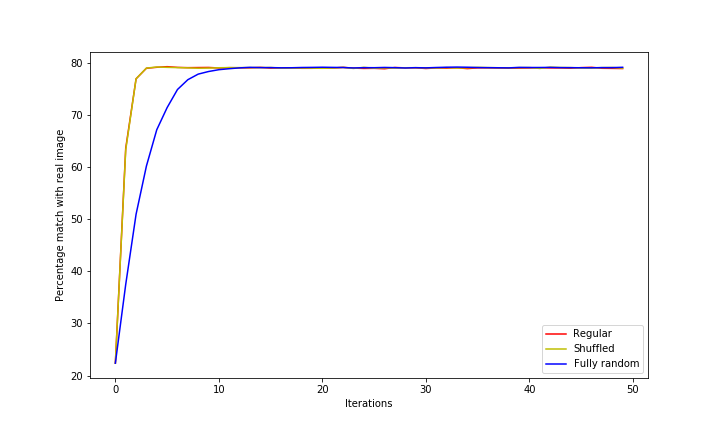
\includegraphics[width=0.48\textwidth]{images/GibbGuassianMatch.png}
    \caption{Graph showing percentage match of different orders for Gibbs applied to our image with Gaussian noise, against iterations}
    \label{fig:GibbOrderComp}
\end{figure}

\noindent\textbf{Question 4}\\
Each approach tends to the same stable point, which in this case, is after approximately 10 iterations. Running past this point yields little or no improvement. The number of iterations to reach this stable point seems to depend on the choice of hyper-parameters - $\eta$ and $\beta$, which also affect the maximum percentage match reached. This problem is then reduced to optimising the hyper-parameters - something that practically is hard, and 'optimised' is dependent upon the bad percentage match metric. 

As we have access to the clean image, it is possible to vary the hyper-parameters and see the effect they have on the results, as in Figure \ref{fig:EtaBetaVariation}. The ratio between $\eta$ and $\beta$ - that is, the ratio of the weights assigned to the likelihood and the prior - seems like the more important factor, not their exact values. Figure \ref{fig:EtaBetaVariation} shows how varying these effects Gibbs' accuracy for a set number of iterations and order. However, different images will be 'optimally' denoised by different choices of $\eta$ and $\beta$, thus optimising these parameters with respect to one image is not a good general approach. If this were being implemented in the real world, these hyper-parameters could be learnt from a training set.\\
\begin{figure}
    \centering
    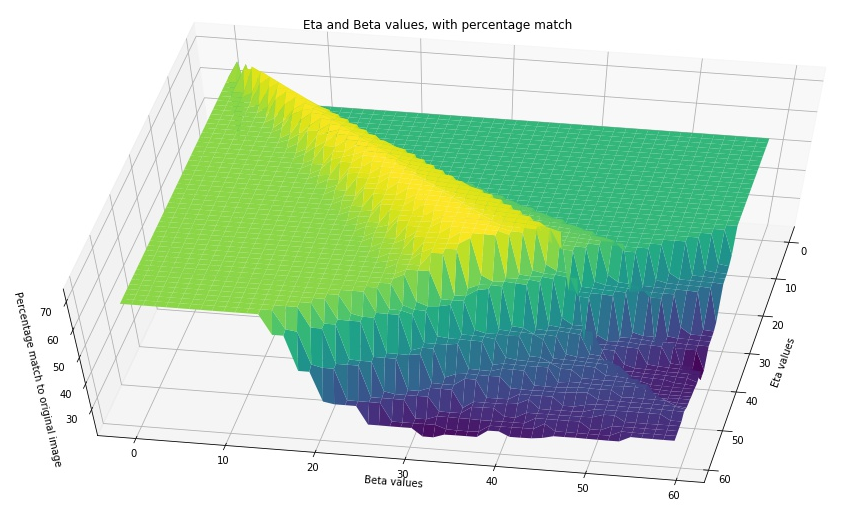
\includegraphics[width=0.48\textwidth]{images/etaBetaResize.png}
    \caption{The effect of varying $\eta$ and $\beta$ on our percentage match, rotated to best show}
    \label{fig:EtaBetaVariation}
\end{figure}

\noindent\textbf{Question 5}\\
There are two main types of KL Divergence \cite{klDiv}.
First we consider reverse KL Divergence as this is what is use in the model, defined in Equation \ref{eq:KL_reverse}.
\begin{equation}
     KL(q(\mathbf{x})||p(\mathbf{x})) =  \int q(\mathbf{x}) \log\left(\frac{q(\mathbf{x})}{p(\mathbf{x})}\right)d\textbf{x}
     \label{eq:KL_reverse}
\end{equation}
This shows that the divergence between \qx and \px is weighted by \qx. This gives most divergence at points where we have a probability mass for \qx and small probability mass for \px. Clearly if \qx  has no probability mass, then the term is zero, and having \px $=$ \qx also gives zero. Having low \px probability mass gives a small denominator, therefore this combined with some \qx mass contributes to divergence. The resulting KL divergence is therefore a measure of how well \qx fits \px where \qx actually has mass, and does not penalise for sections of \px for which \qx is zero.  

Now consider forward KL divergence - in Equation \ref{eq:KL_forward}.
\begin{equation}
     KL(p(\mathbf{x})||q(\mathbf{x})) = \int p(\mathbf{x})\log\left(\frac{p(\mathbf{x})}{q(\mathbf{x})}\right)d\textbf{x}
     \label{eq:KL_forward}
\end{equation}
Forward KL weights the integral with \px, rather than reverse KL which uses \qx. This means that divergence increases anywhere \px has probability mass, and is increased by low \qx as we are dividing by \qx. This gives large divergence if there are sections of the \px distribution that \qx does not approximate at all, which is - as you'd expect - the opposite of the reverse case. This measure does permit \qx to have extra probability mass far away from \px and this does not count towards divergence, which is the reason this is not useful in our case.\\

% The difference between these we can also write out, as in Equation \ref{eq:KL_difference}.


% \begin{align}
%     &\int q(\mathbf{x}) \log\left(\frac{q(\mathbf{x})}{p(\mathbf{x})}\right)d\textbf{x} - \int p(\mathbf{x})\log\left(\frac{p(\mathbf{x})}{q(\mathbf{x})}\right)d\textbf{x} \nonumber \\
%     &= \int q(\mathbf{x}) \log q(\mathbf{x})d\textbf{x} + \int p(\mathbf{x}) \log q(\mathbf{x})d\textbf{x} \nonumber \\
%     &\ - \left( \int q(\mathbf{x}) \log p(\mathbf{x})d\textbf{x} + \int p(\mathbf{x}) \log p(\mathbf{x})d\textbf{x} \right) \\
%     &= \int \left( p(\mathbf{x}) + q(\mathbf{x})\right) \log \left( \frac{q(\mathbf{x})}{p(\mathbf{x})}\right)d\textbf{x}
%     \label{eq:KL_difference}
% \end{align}

\noindent\textbf{Question 6}\\By using a mean-field approximation, it is assumed that the approximate distribution over each latent variable is independent. This means that each latent variable is entirely parameterised by an independent parameter $\mu_i$. In the case of image inference, one simply needs to find the appropriate values of $\mu$ to find a suitable approximating distribution for the pixel's value.

Each of these parameters are calculated using equation \ref{eq:variational}.

\begin{equation}
    {\mu}_{ij}^{\tau+1} = tanh\left(\sum_{{kl}\epsilon\mathcal{N}(ij)} \omega_{ij}\mu_{kl}^\tau + \frac{1}{2}\left[L_{ij}(1) - L_{ij}(-1)\right] \right)
    \label{eq:variational}
\end{equation}

The first term is the sum of the weighted values of the pixels in the neighbourhood. This term is positively large if the neighbourhood is primarily in agreement with the centre pixel, and negatively large if they are primarily in disagreement. This fits with our intuition, as a positive large value evaluated with $tanh$ will give a value of $1$, similarly $tanh$ will return $-1$ when evaluated with a large negative value. When the pixels in the neighbourhood do not belong primarily to one class, then the summation in Equation \ref{eq:variational} is much smaller. As a result the parameter $\mu$, when updated, is affected less by the prior.


The second term in Equation \ref{eq:variational} is the difference in likelihood of the ij\textsuperscript{th} latent pixel being white or black respectively. This term is large when the observed pixel is white and small when it is black.

In Figure \ref{fig:variationalBayes}, it can be seen that the Variational Bayes method performs exceptionally well for Gaussian noise corruption, but less so for "Salt and Pepper" noise. Experimenting with different values of $\beta$ and $\eta$ (in this case weighting the left and right terms respectively) and, one could alter how well Variational Bayes performs with the different noises. One configuration of $\eta$ and $\beta$ could perhaps perform well with Gaussian noise and performs poorly with Salt and Pepper noise whilst another configuration could do the complete opposite.\\

\begin{figure}
    \centering
    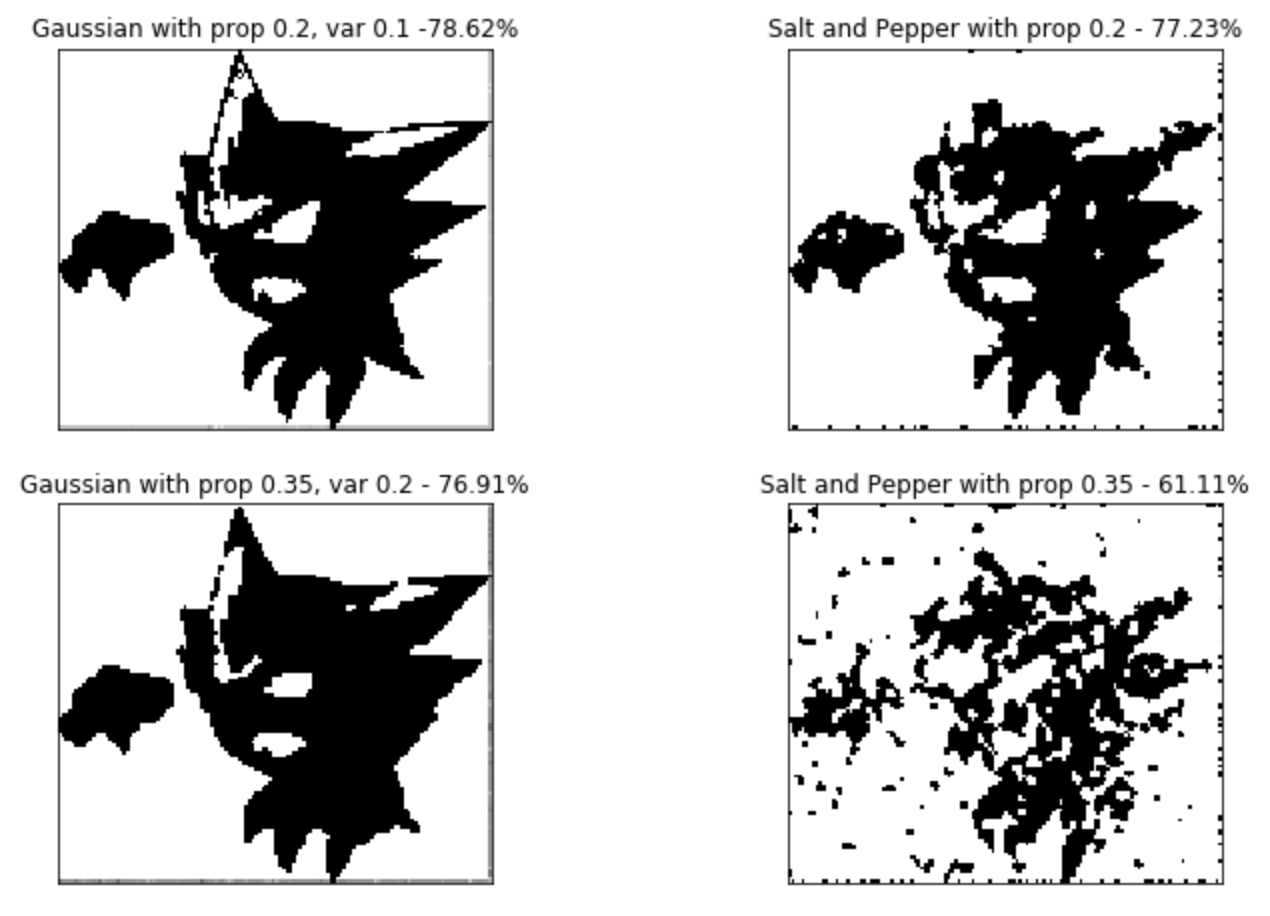
\includegraphics[width=0.48\textwidth]{images/variationalBayes.png}
    \caption{Variational Bayes by Ising Model}
    \label{fig:variationalBayes}
\end{figure}

\noindent\textbf{Question 7}\\
So far we have outlined and assessed the performance of the three approaches to image denoising, but only in isolation. Comparing the different approaches allows for assessment of the relative performance of each model, as well as the relative benefits and setbacks. Gibbs sampling is a stochastic approach. Both variational Bayes and ICM are deterministic, however the former is much more sophisticated in its approach. When comparing the different approaches, it is useful to compare under two categories: time taken to converge, and accuracy. The question to ask is whether or not we must sacrifice accuracy in order to achieve efficiency? 

\noindent \textbf{Time taken to converge:}
 From figures \ref{fig:MethodComparisonChanges} and \ref{fig:MethodComparisonMatch}, we see both ICM and variational Bayes converge faster than Gibbs. It was proved earlier using the monotone convergence theorem that ICM is guaranteed to converge to a local maximum. Convergence of Gibbs is also guaranteed, as shown in this paper \cite{roberts1994simple}. However, Gibbs took much longer to converge than both ICM and variational Bayes. 
 \begin{figure}
     \centering
     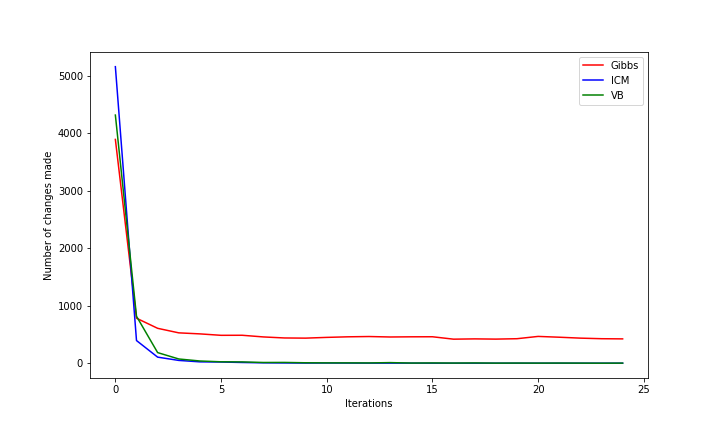
\includegraphics[width=0.48\textwidth]{images/AllComparisonChanges.png}
     \caption{Number of changes made by each method over iterations}
     \label{fig:MethodComparisonChanges}
 \end{figure}
 \begin{figure}
     \centering
     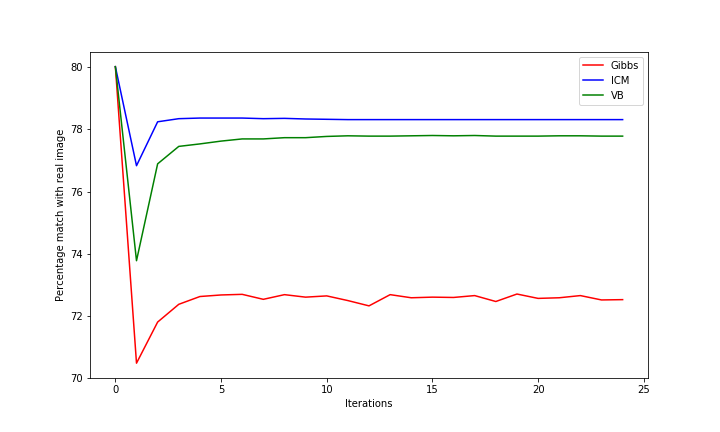
\includegraphics[width=0.48\textwidth]{images/AllComparisonMatchSnP.png}
     \caption{Percentage match for each method over iterations}
     \label{fig:MethodComparisonMatch}
 \end{figure}

\noindent\textbf{Accuracy:}
The accuracy of each approach was measured by percentage of pixels that matched the original image upon termination. From figure \ref{fig:MethodComparisonMatch} we see that ICM and Variational Bayes out-perform Gibbs when the image is corrupted with salt and pepper noise. However, this graph is based on a partly-flawed metric and does not reflect how good the image may look to a human. 
To fully understand why Gibbs behaves the way it does, it is useful to understand how it explores the posterior manifold mentioned earlier. Gibbs samples from the posterior and, unlike variational inference, Gibbs is theoretically capable of exploring the entire support of the manifold. The support of a manifold is just those elements which are not mapped to zero (areas that have a non-zero probability mass in our case). Gibbs should then, theoretically, be able to reach a global optimum. However, it would take a long time to do so as Gibbs is computationally expensive. Any modest restriction on the time for which the sampler is running ensures that Gibbs can only explore a localised area of the support and thus cannot find a global optimum.

Variational Bayes, on the other hand, uses approximations of distributions and is thus not capable of finding a global optimum. As a result of this, Gibbs should theoretically out perform variational Bayes if given sufficient run time.

While our data implies that Variational is more accurate than Gibbs over a short time frame, we are skeptical of this result as there is still uncertainty in the literature as to which method is more accurate. The following is an excerpt from a paper by Blei and Kucukelbir and McAuliffe: "Variational Inference: A Review for Statisticians" \cite{Blei2017Review}://
"The relative accuracy of variational inference and MCMC is still unknown. We do know that variational inference generally underestimates the variance of the posterior density; this is a consequence of its objective function. But, depending on the task at hand, underestimating
the variance may be acceptable. Several lines of empirical research have shown that variational inference does not necessarily suffer in accuracy, e.g., in terms of posterior predictive densities (Blei and Jordan, 2006; Braun and McAuliffe, 2010; Kucukelbir et al., 2016); other research focuses on where variational inference falls short, especially around
the posterior variance, and tries to more closely match the inferences made by MCMC (Giordano et al., 2015)."\\
\\
\noindent\textbf{Gibbs Sampling or Variational Bayesian Inference?}
Taking all of this into account, when should one use variational Bayes and when should one use Gibbs, or any other MCMC method? Gibbs is computationally more intensive but can guarantee asymptotically exact examples. Variational Bayes can only give an approximation, but is in general much faster than Gibbs. As variational Bayes can be reduced to an optimisation problem (minimising the KL-divergence), it can make use of optimisation methods, such as those outlined in this paper: \cite{herbrich2005minimising}, to more efficiently approximate the posterior distribution.\\
\\
\noindent\textbf{The best of both worlds:}
Given the apparent trade-off that one must make between efficiency and accuracy, it is natural to ask whether or not it is possible to combine the two approaches for better results. This paper \cite{salimans2015markov} titled "MCMC and Variational Inference: Bridging the Gap" (reference paper), outlines the possible ways in which the two approaches could be synthesised to give "fast posterior approximation through the maximisation of an explicit objective, with the option of trading off additional computation for additional accuracy."

%----------------------------------------------------------------------------------------
%	BIBLIOGRAPHY
%----------------------------------------------------------------------------------------



\printbibliography[title={Bibliography}] % Print the bibliography, section title in curly brackets


%----------------------------------------------------------------------------------------

\end{document}
